\documentclass{amsart}


\usepackage{amssymb}
\usepackage{amscd}


\usepackage{graphics,amsmath,amssymb}
\usepackage{amsthm}
\usepackage{amsfonts}
\usepackage{latexsym}
\usepackage[pdftex]{graphicx}
\usepackage{float}



\renewcommand{\refname}{}


\title{Title}

\begin{document}
\DeclareGraphicsExtensions{.pdf,.png,.gif,.jpg}
\bibliographystyle{plain}
\maketitle

\section{\bfseries{Introduction}}
	\subsection{Background}
		All countries implement a set of rules that help to regulate traffic and essential determine the common practices of the roads.  Many times though drivers choose to vary their compliance with all of these rules.  This disregard usually stems from drivers personal feelings on whether a rule is effective, if the rules conditions annoy the driver, and perceived time saved by breaking the rule.  One of these rules that has varying compliance is the rule that states a driver has to stay right unless to pass.  This states that a driver can only pass on the left of a driver and once they pass they should return to the right lane once they can.  Compliance is the key factor in the implications and effectiveness of this rule.  The question to be tested though is if people are going to follow this rule will it actually increase efficiency and safety of traffic flow. 
	
	\subsection{Approach}
		In order to test how efficient this rule is for traffic flow and safety, we needed to first establish a model for how our traffic is interacting and how the traffic is flowing as a whole. Essentially in order to test if the rule has an effect we cannot check already existing data but instead create our own data that is models a controlled variation in rule application. The currently most popular modeling of traffic involves treating the whole system as a pipe with fluid and then applying the discoveries and theorems of fluid dynamics.  This model is a macroscopic model though where essentially all control and measuring of the individual interactions is lost.  The other most common modeling technique for traffic flow is with individual particle interactions.  This treats each car, sometimes groups of cars, as a single particle and analyzing how these particles interact.  Our computer model turned out to be a particle model that treats each car as an individual.  Once we develop the system to analyze each individual interaction on a road system then we can begin to change how a driver will respond to this interaction.  As we vary these interaction choices, such as stay right except to pass or pass whenever and wherever you can, then we can see what the results of each interaction decision will have on the effect of the system as a whole.  

\section{\bfseries{Assumptions and Definitions}}
	\subsection{Definitions}
		\begin{itemize}
  			\item \textit{Highway}:an ideal model of a road with no entries or exit points
			\item \textit{Vehicle}:an ideal car that has all share same constant length 
			\item \textit{Driving Lane}: a highway lane a vehicle is free to travel in
  			\item \textit{Passing Lane}: a highway lane a vehicle can only travel in while passing
			\item \textit{Travel Time}: the time needed for a vehicle to travel length of road
			\item \textit{Traffic Flux}: the rate of cars passing a single location along the highway
			\item \textit{Rule}: distinct formulations of the passing laws 
			\item \textit{Side-Swipe Accident}: collision based solely on lane-changing
			\item \textit{Read-End Accident}: collision based solely on inefficiency to slow down
			
		\end{itemize}
	
	\subsection{Assumptions}
		General assumptions to the problem turned out to be one of the biggest road blocks that influenced our progress.  At each step in both the method choosing and the model developing we had to evaluate previous assumptions we had made and what further assumptions we would need to make in order to promote realistic situations while still having a solvable system.  There were some major overlaying assumptions that we made:
		\begin{itemize}
			\item  	Discrete Velocity and Discrete Position
			\item  Hot Air Balloon Perspective
			\item 	All vehicles have the same length 
			\item 	Internal vehicular performance does not vary
			\item  Lane width, shoulder width, and curvature of road do not effect highway dynamics
			\item 	Conservation of Cars: Total Number of Cars on Road Constant
			
			\item  	All roads are uninterrupted highways
				\begin{itemize}
					\item 	No vehicles enter midway through road
					\item 	No stops in highway allowed (traffic lights/intersections) 
				\end{itemize}
			\item   Crashes have no effect on dynamics of highway
			\item 	Severity of Side Swipe accidents equal to severity of Rear-Ending accidents			
		\end{itemize}
		 

		To allow the model to be programmed we had to make the simplification that velocity and positions of vehicles were both discrete quantities.  There are two reasons this is reasonable: snapshots of highway and ability to scale.  The discrete speeds and positions can be interpreted as snapshots of the highway at constant intervals.  This says that within our program each iteration is simply a snapshot of how the highway is performing at each period of time.  If we then scale the position spacing size down each iteration will represent smaller and smaller time periods.  This shrinking of time intervals is similar to the idea of a video being simply a sequence of photos changing at a fast speed.  As for velocity, once we have discrete positions velocity can only be assigned in quantities of those discrete positions.  If position spacing was scaled down then velocity could be rescaled in terms of the new position interval in order to get more continuous velocity options. 
	
		Hot Air Balloon Perspective is a perspective assumption based on a view of the whole section of the highway at a single time instead of an internal perspective where we are measuring from inside the system.  This plays into both the programming of the model as well as the macroscopic measuring of the system. 
		
		A constant vehicle length can be defined due to only slight variations in actual car length. Also, since there are discrete position intervals, a car can only be integer lengths of these discrete position intervals. As for modeling longer vehicles, the model can allow two constant length vehicles to be connected in line at a specific speed.

		Internal vehicular performance is in reference to that all cars break, accelerate, and function at equal levels.  This assumption is a more subtle point that would increase variable amount without increasing the benefit of testing the passing rules.  Also, by the assumption that cars travel at discrete constant velocities internal vehicular performance should not vary on a vehicle to vehicle basis.   

		Lane width, shoulder width, and curvature of the road are assumed to have no effect on the testing of the passing rules.  In general, lane widths on a highway have such small variations that any difference is assumed to have nominal effect on the ability to switch lanes.  Also, smaller lanes allow faster lane changes but decrease traveling safety so the assumption is these small variations do not affect safety.  (SOURCE) Same principles go apply to highway shoulders and median variations. No oncoming traffic is assumed so the median consideration is unnecessary at this time.  Shoulder width is seen to have an effect on a driver’s safety perception but is assumed to have insignificant effect on efficiency of a passing rule application (SOURCE).
		 
		 Conservation of cars is a combination of factors: no vehicles enter mid-way through the highway and the density of the entire road as a whole is constant.  This correlates to there being no exit or entry ramps in this stretch of the highway and that as a car exits the highway a car enters the highway.  This assumption is essentially a simplification for programming the model because we need a way to add new cars to the highway but generating new cars after each iteration would not provide enough benefit for the use of our programming time frame. As the length of the highway is increased though the inaccuracies decrease because it takes longer for a car to pass the same vehicle twice.  To further justify this assumption reference can be made to large percentage of traffic models that do in fact make this assumption (SOURCE).  
		 
		 In our definition of a highway the assumption was already made that there are no exits or entry ramps midway through the highway.  Further we want to exclude any slowing or stopping due to traffic lights, intersections, or further impairments since these should not have an effect on the specific testing of the passing rules.  Our model allows for these adjustments to be made with minimal code writing but once again the time to write it wouldn't be beneficial enough to test these specific passing rules.  

		In our model we calculate the amount of accidents that are likely to result on a highway but simultaneously assuming that a crash will not stop or slow down traffic.  One main reason for this assumption is to make the programming simpler, since an accident is simply a number count in the program.  More importantly though, the assumption is justified because we want to test crashes caused simply by these passing rules.  When crashes are allowed to slow down traffic, the model begins to add accidents do to the slowing and increasing density of traffic and not directly the passing rules themselves.  

	Although there are different probabilities associated with side-swipe accidents vs. read-end accidents no severity of crash time is assigned.  That implies that the safety of the highway is not associated with how bad accidents on the highway actually are.  This could be later factored in but there are too many variables to associate a severity of an accident to program a severity calculator in this time.  This assumption is also reasonable because even non-severe accidents should  be prevented. 
		


\section{\bfseries{Development of Method}}
	\subsection{Method Rational}
	Our approach to testing passing rules was to develop an effective model for traffic interactions that could create it's own data depending on the set of rules for the road that we wanted implicated.  This would then allow more control over parameter variation instead of simply relying on already collected data by others for a specific highways with a specific rule.  Furthermore, if we were able to build a model that had very specific parameter variation capabilities then the analysis of the road rules would be easier to analyze and interpret since we could run rules against control situations.  
	
	
	
	Initially there were three general model ideas that we considered in order to create these rule data variations. The first was a single particle model that would effectively model each individual interaction of a car trying to pass another car.  The other extreme was the macroscopic idea, modeling the highway as a whole, to use differential equations to model the rate of flow for traffic.  Inside the idea of differential equations, fluid dynamics and it's associated differential equations were discovered to be of significant current use in modeling traffic flow.  The third model we considered developing was some form of a combination of the particle model and fluid dynamics model. 
		
		\subsubsection{\it Fluid Dynamics}
		In the realm of macroscopic traffic modeling, fluid dynamics is the most popular and common technique.  The idea behind this technique is that cars in heavy traffic interact similar to particles, either gas or liquid, in a confined tube.  
The difference between gas and liquid being the property of compressible, or the ability to change density of the fluid.  A gas model is said to be compressible, allowing changes in  fluid density.  While a liquid model is said to be incompressible, allowing no change in fluid density(JP SOURCE: MCM RESEARCH SOURCE FLUID DYNAMICS).  The majority of fluid dynamical models that we considered used incompressible calculations on both a macroscopic and microscopic model.  Our first approaches involved attempting to vary viscosity within the fluid and vary the shape of the tube the fluid traveled through.  By varying viscosity then the high viscosity pockets of fluid would represent slow pods of traffic while low viscosity fluid would represent fast moving pods of traffic.  The other technique called slow traffic pods an actual unmovable obstruction as part of the pipe wall or shape.  
		
		
	
	
	
		
		\subsubsection{\it Discrete Particle Model}
		
	The other extreme of modeling that we tried to pursue involved a discrete particle model that monitored individual interactions.  In this model we were hoping to create a program in detail that modeled specific passing characteristics of interactions.  By evaluating the actual different parameters that make up every passing interaction then these would shed light on the efficiency of the stay right except passing rule.  This model would be able to measure the safety of passing on the right vs. passing on the left, amount of time required for each passing interaction, the effect passing had on the immediate properties of each vehicle, etc.  
	Within this model though you start to lose sight of the overall highway as a whole.  By simply considering a few interactions at a time it's almost impossible to see traffic jams develop, highway flow changes, or density of the highway.  If we couldn't test these factors then it would be hard to say whether the different passing rules had any large effect on the efficiency of the highway system as a whole.  
		
		\subsubsection{Mixed Model}
		
	Eventually the obvious conclusion was to attempt to find an effective median between macroscopic fluid dynamics and the individual discrete particle model.  Along with this though we decided to start with the discrete particle model and slowly generalize it into a more macroscopic situation.  By utilizing the particle model still we had an effective way to vary the actual interaction between every single car.  This gave us complete control over what actually happens when a car tries to pass another car.  
	
	The very first model that we fully developed was a short programming code that gave us data we could then illustrate on graph paper.  This original program only had a road length of 100 tiles, with discrete tile position and speed based off of tiles per iteration of the program.  As we drew out the positions we began to discover not only the bugs in our program program but also in the short length of road and vehicular speed classes of 1,2,3 tiles/iteration.  We were able to further understand which aspects of each passing interaction we considered the most important and these began the factors of test in our final method.  

	\subsection{Discrepancies of Fluid Dynamics}
	The major problem right away with fluid dynamical modeling was creating a solution to implement a passing rule into the fluid's attributes. Since we were unsuccessful in finding an already existing model that allowed for this variation in passing rule, the technique we pursued was implementing a system containing a fluid with non-unified viscosity. 
	
	One problem that appeared with using fluid dynamical techniques was the models accuracy to model traffic decreases as density decreases (SOURCE JP PDF FLUID DYNAMICS).  This is in effect because as density decreases there begins to appear these large gaps in traffic that would not be present in either a liquid or a gas, even if we allowed the fluid to be a compressible fluid.  One variation in parameters that we consider important for testing was the passing rules efficiency in both low and high density. Some models attempted to adjust for density by varying viscosity of the fluid as we had hoped.  In these cases though the differential equation analysis became more and more complicated as the viscosity varied.  Since we felt our model required large variations in viscosity in small intervals we were led to the conclusion that all these models assumptions generalized the fluid into too macroscopic of a model to test any passing rule interaction of vehicles effectively.    

	We further investigated other theories in the fluid model however found that simply none allowed the use of a particle specific rule that we felt comfortable enough quantifying as a passing rule, thus preventing us from using them to answer the basic problem statement \cite{piccolireview}.
	
	\subsection{Choosing Final Model}

\section{\bfseries{Road Rules}}
	The rule that staying right except to pass becomes a more subtle point as the highway becomes three or more lanes wide.  Essentially there are two different rules that this stay right rule breaks down into when three or more lanes are present.  There is the rule that all drivers must remain as far right as possible and the rule that there is a single left most passing lane and drivers can travel within the remain other lanes freely.  In order to test all variations in passing tendencies four separate passing rules were developed:
		\begin{itemize}
			\item No Passing Allowed
			\item Free Passing
			\item Single Passing Lane
			\item Single Driving Lane
		\end{itemize}
	These are the four different rules of passing that we decided to test within our model.

	\subsection{No Passing Allowed}
	The No Passing Allowed Rule states that all lanes on the highway are driving lanes and that there is no passing involved in the system at all.  Under this rule whatever lane a vehicle starts within the vehicle will remain in that lane for the entirety of its travel.  The obvious result of this system is that quickly there will be large chains of cars all going at the same speed.  When the two or more lanes are present on a stretch of highway this model has no practical application, which supports why we are developing it as a control rule.  There are applications to this rule though when the highway only has one lane traffic, as in a construction zone or on a highway where there is only one lane traffic in each direction and the oncoming traffic is too heavy to ever pass.  In these cases, this No Passing Allowed Rule can provide effect insight into the clustering of these speed pockets.  Our research question isn’t concerned with this case of speed pockets though so we will simply think of this No Passing Allowed Rule as a base case that represents an extreme in the spectrum of rules.  
	\subsection{Free Passing}
	The Free Passing Rule states that the vehicle will continue in its current lane until it approaches another vehicle in its lane.  At the point that another vehicle is in front of the target vehicle the target vehicle will attempt to change lanes.  The vehicle will first try to pass the front vehicle on the left, but if there is no lane open to the left then the vehicle will attempt to also pass to the right.  If passing is also not possible to the right then the car will slow down to mirror the speed of the vehicle it is following. 

	Therefore there are two important differences in this rule then in the other rules, direction of passing and the action after lane changing.  Under this rule vehicles can pass going either to the left or to the right.  Also, once a vehicle does change lanes it will remain in that lane until it is forced to pass again.  

	This rule is providing us with a model that shows the absence of any passing laws.  In practical application most cars don’t operate by this Free Passing Rule, but there are certain individuals who interact in this manner when they feel they need to.  The real importance of this rule is that it provides a control case on the other extreme of the rule spectrum opposite that to the No Passing Rule.  The Free Passing Rule says that there is an absence of any rules regarding passing and thus gives a basis to show that passing rules need to be implemented to improve efficiency and safety. 
	
	\subsection{Single Passing Lane}
	The Single Passing Rule states that there is only a single passing lane on the multilane highway and the remaining lanes are designated as driving lanes.  A Single Passing Rule and a Single Driving Rule are equivalent on a one or two lane highway.  This rule was created in order to account for the travel of slower vehicles in more than just the farthest right lane for highways of more than two lanes.  Therefore any lane that is not the farthest right or the farthest left lanes allows both driving and passing within it. 
	
	This rule can be assumed to closed mirror how heavy traffic flow works on a busy multilane highway.  Drivers tend to spread out among multiple lanes spending more time in a lane the farther right that lane is on the highway and leaving the left lane frequently empty or for carpooling.  We have not including any regard for a carpool lane since in our program only fast drivers will be traveling in the left lane at any time.   
	
	\subsection{Single Driving Lane}
	The Single Driving Rule states that the farthest right lane is a driving lane and all other lanes on the highway are only passing lanes.  A Single Driving Rule and a Single Passing Rule are equivalent on a one or two lane highway.  

	This rule tests the stay right except to pass law most efficiently.  By forcing drivers to only travel in the right lane except while passing the system takes into effect that a vehicle has to return to the same lane they were previously traveling in before overtaking another vehicle. Therefore this rule must be tested against the efficiency and safety of all the other rules in order to actually test the stay right except to pass law.    

\section{\bfseries{Modeling}}

\textit{\textbf{Model Specific Definitions}}

\begin{itemize}
	\item \textit{Initial Speed}: speed of individual vehicle at start of simulation
	\item \textit{Current Speed}: speed of individual vehicle at individual time	
	\item \textit{Iteration Average Speed}: the average current speed of all vehicles on the highway
	\item \textit{Highway Density}: amount of cars over whole highway; constant in current model
	\item \textit{Traffic Flux}: the average speed multiplied by the highway's density
	\item \textit{Road Type}: initial conditions of a highway based on density (high or low) and lane count (2-5)
	\item \textit{Simulation}: total iterations for all possible road type	
	\item \textit{Average Simulation Speed}: the average speed for a certain road type simulation
\end{itemize}
	
\textit{\textbf{Model Specific Assumptions}}

	\begin{itemize}
	\item Normal Distribution of Initial Speed
	\item Speed Increases to Initial Speed When Possible
	\item All overlying assumptions stated previously
\end{itemize}

\textit{Justifications}\\


	
	
	
	Initial speed of the vehicles on the highway was chosen by a normal distribution.  This assumption was actually made to maximize the realism of our method.  Speeds in the current scaling of the system are taken to range from 54 MPH to 90 MPH.  This sets the average speed of the highway at 70 MPH which is a common speed limit for United States highways.  By normally distributing initial speeds the break downs are:
	
	\begin{figure}[h]
\begin{center}
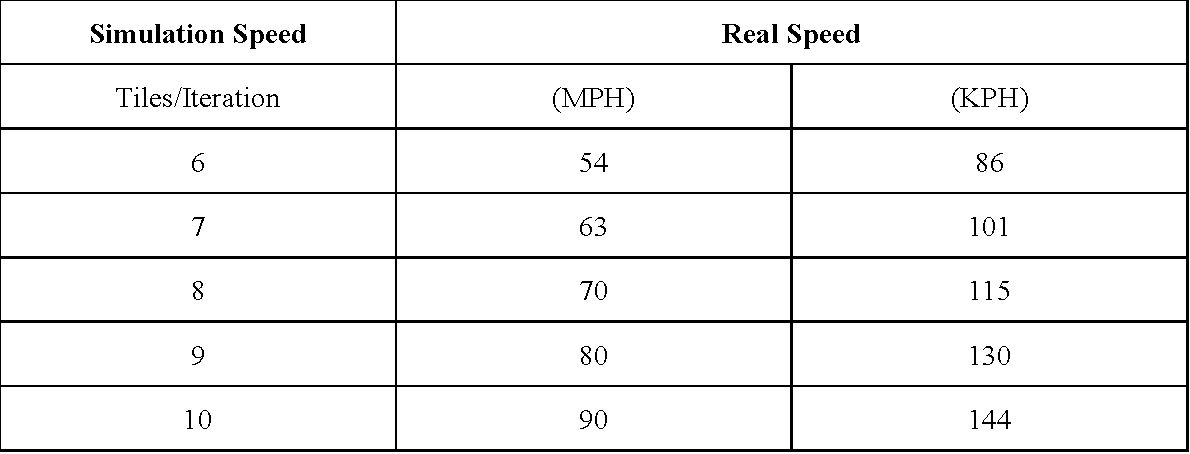
\includegraphics[scale=0.5]{MCM-SimulationSpeedTable.pdf}
\caption{Comparison scale of speed within model to the representation in real speeds.}
\renewcommand{\figurename}{Speed Scaling}
\end{center}
\end{figure}

	Inside the simulation vehicles are often slowing down since no crashes are allowed in the system.  Therefore we assume that every vehicle wants to accelerate back to it's initial speed as soon as it possibly can.  This is an important assumption in the realism of the method because on real highways individual drivers tend to drive at a steady average speed when their path is not impeded.  
	
	\begin{figure}[h]
\begin{center}
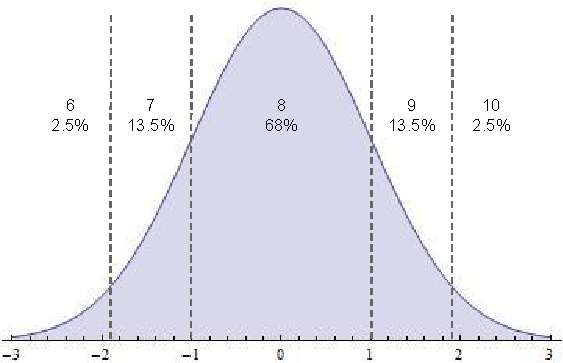
\includegraphics[scale=0.65]{MCM-speedsnormaldist}
\caption{Normal distribution graph of initial speed.}
\renewcommand{\figurename}{}
\end{center}
\end{figure}
	
	\textbf{INSERT SHORT TABLE HERE FOR INITIAL DISTRIBUTION!!!! AND MAYBE NORMAL DISTRIBUTION GRAPH WITH INTEGER SPEEDS ADDED IN AS WAS DRAWN ON THE BOARD}  
	
	\subsection{Description of Model}
	
	
	\subsection{Logic Structure}
	
	\textbf{INSERT LOGIC TREE HERE!!!}
	
	\begin{figure}[H]
	\begin{center}
	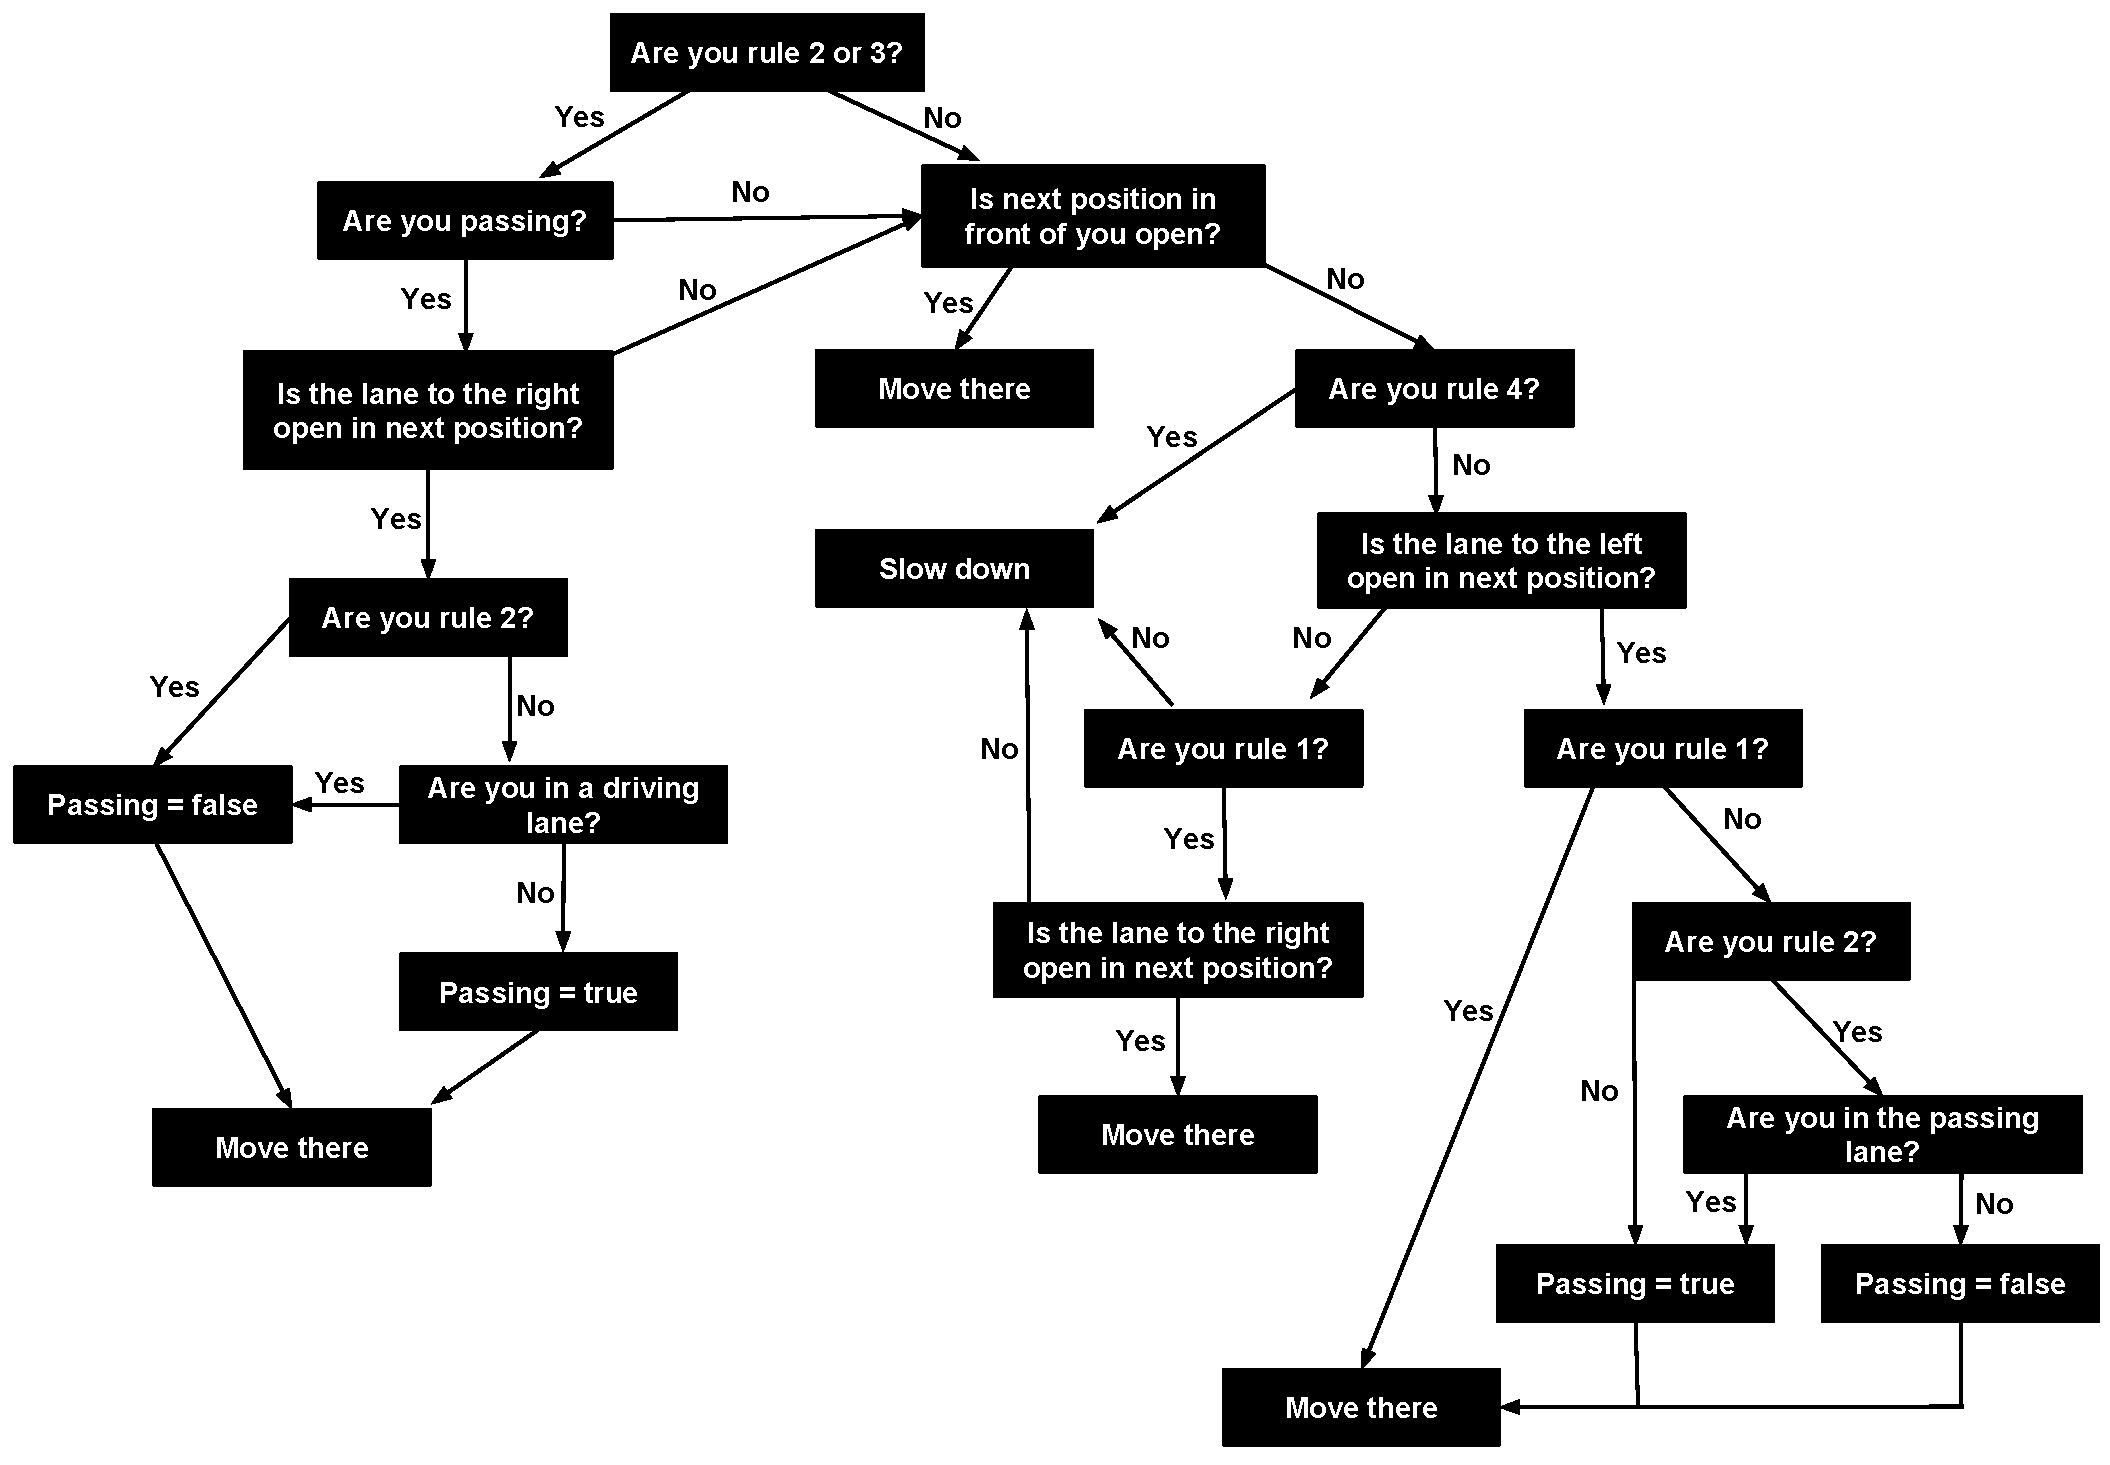
\includegraphics[scale=0.4]{MCM-LogicalFlowChart.pdf}
	\caption{The Logic Flow Chart of the programming sequence.}
	\renewcommand{\figurename}{}
	\end{center}
	\end{figure}
	
	\begin{figure}[H]
	\begin{center}
	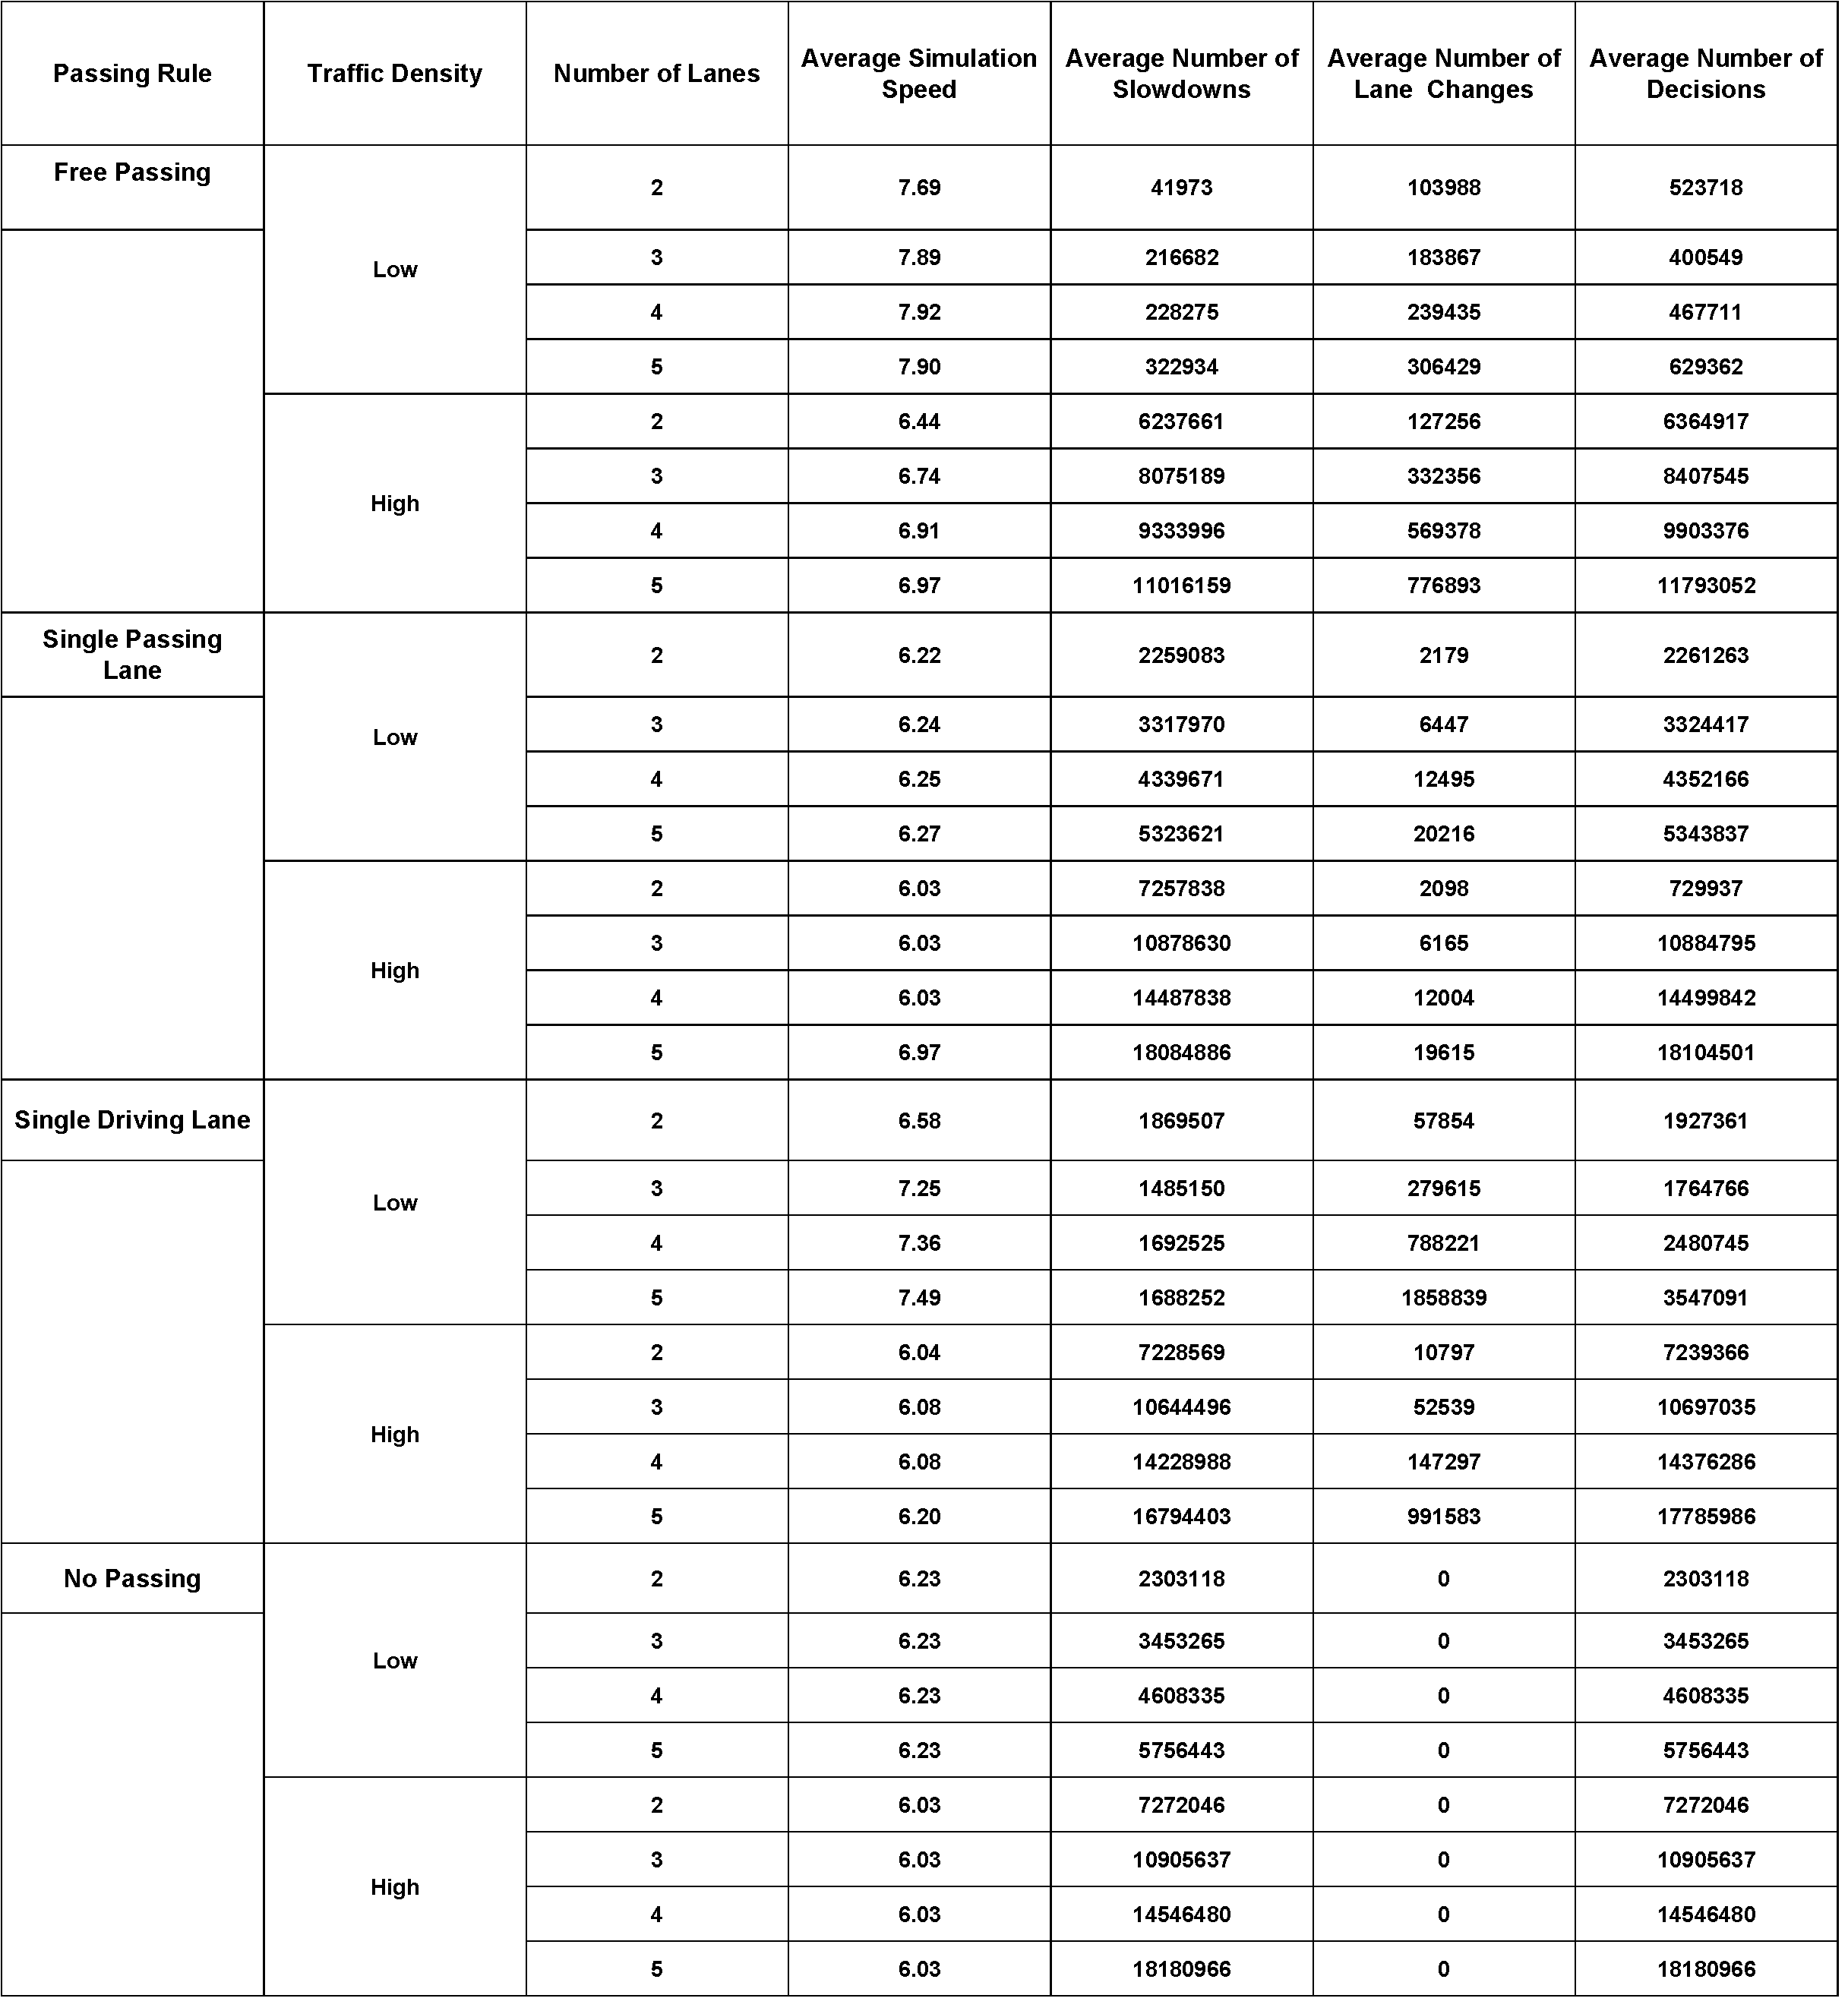
\includegraphics[scale=0.3]{MCMDataSummary}
	\caption{Program's computational outputs.}
	\renewcommand{\figurename}{}
	\end{center}
	\end{figure}
	
	\subsection{Coding of Program}
	
	\textbf{INSERT IMPORTANT CODE LINES IF THERE ARE ANY!}

\section{\bfseries{Analysis of Rules}}
	\subsection{Applying Rules}
	\subsection{Data from Model}
	
	

\section{\bfseries{Statistical Analysis}}
	\subsection{Assumptions and Definitions}
	\subsection{Statistical Test Choice}

\section{\bfseries{Results}}

\section{\bfseries{Strengths and Weaknesses}}

(EXPLAIN WHY CHECK CLEAR PATH COULD OF FAILED US!)
(Check to make sure that the vehicles are speeding back up properly.  Since most cars are traveling at a speed of 6 for the majority of their travel.) 
(Some problem in probability of accident analysis.  Is conditional probability viable in this case? What about when P(s) and P(l) approach zero, then the P(A) goes to infinity. What's going on?) 

\subsection{Strengths}

\textbf{HOW REALISTIC IS OUR MODEL?}

\subsection{Weaknesses}

The optimal travel time vs. actual travel times for individual cars.

  

\section{\bfseries{Conclusion}}

\section{\bfseries{Future Work}}
	With the development of our program there are opportunities to adjust the starting conditions and individual vehicle interactions.  Therefore the programs parameters can be changed in order to make the model more practical to the real world or to test different traffic flow questions.  With this ability in our model some variations should be tested but could not be completed within the time frame.  
	\subsection{Car Individualized Rules}
	(INSERT something about how slow cars actually start in the fast lane and can get stuck there for long period of time. Justified by assumption though that they will eventually get over so not sure if want to include or not.)
	\subsection{Psychology Driver Variation}
	One model found attempted to test individual driver psychology of driving.  This acts as a subdivision of the varying speed adjustment.  Driver's may be influenced by perceived safety, age, likelihood to be distracted, emotional distress, etc.  Furthermore in this psychology of individual drivers there is the consideration that drivers can only perceive in a limited viewing frame and thus only varying their speed by the vehicles around them ~\cite{burghout2005}.  These are attributes that can't easily be incremented into our program but would be interesting to pursue if with a small set of simple assumptions our program could begin to describe some of these variations.     
	
\cite{stone2007introduction}




\newpage
\section{\bfseries{References}}
\bibliography{References}











\end{document}
